\section{Link Analysis}

Will a wireless link from $A$ to $B$ work? What speeds can be
expected? How much transmit power is necessary and what kind of
antennae should be used? To answer these questions we do a link budget
calculation. This is,
\begin{equation}
  \label{eq:link_budget}
  P_r = P_t + G + L
\end{equation}
or, the received power is equal to the transmit power, plus gains, and
minus losses. We then check in the manufacturer's table to see if the
received power is sufficient to maintain a link and at what speed.

The main difficulty is in figuring out what $L$ is, because there are
lots of different sources of loss, for example:
\begin{itemize}
  \item cable loss caused by electrical resistance of a feedline
    between  between the radio and the antenna
  \item insertion loss caused by the use of connectors to attach the
    feedline
  \item path loss caused by the spreading out of energy in space (this
    is your ``inverse-$r^2$'' loss)
  \item path loss related to the decreasing ability of an antenna to
    ``hear'' radio waves as the frequency increases (this loss is
    proportional to the square of the frequency)
  \item multi-path loss where two signals from
    the same transmitter follow different paths to the receiver and
    interfere destructively with one another
  \item absorption, primarily by water in the air such as rain and
    fog, but also at higher frequencies by elements such as oxygen and
    nitrogen an effect which varies depending on frequency.
\end{itemize}

To see how this works, let us take a specific example, the link from
Eigg to Ranachan and supposing that the link was to be done with our
common Ubiquiti Rocket M5 radios and dishes. 

\begin{figure}[h]
  \begin{center}
    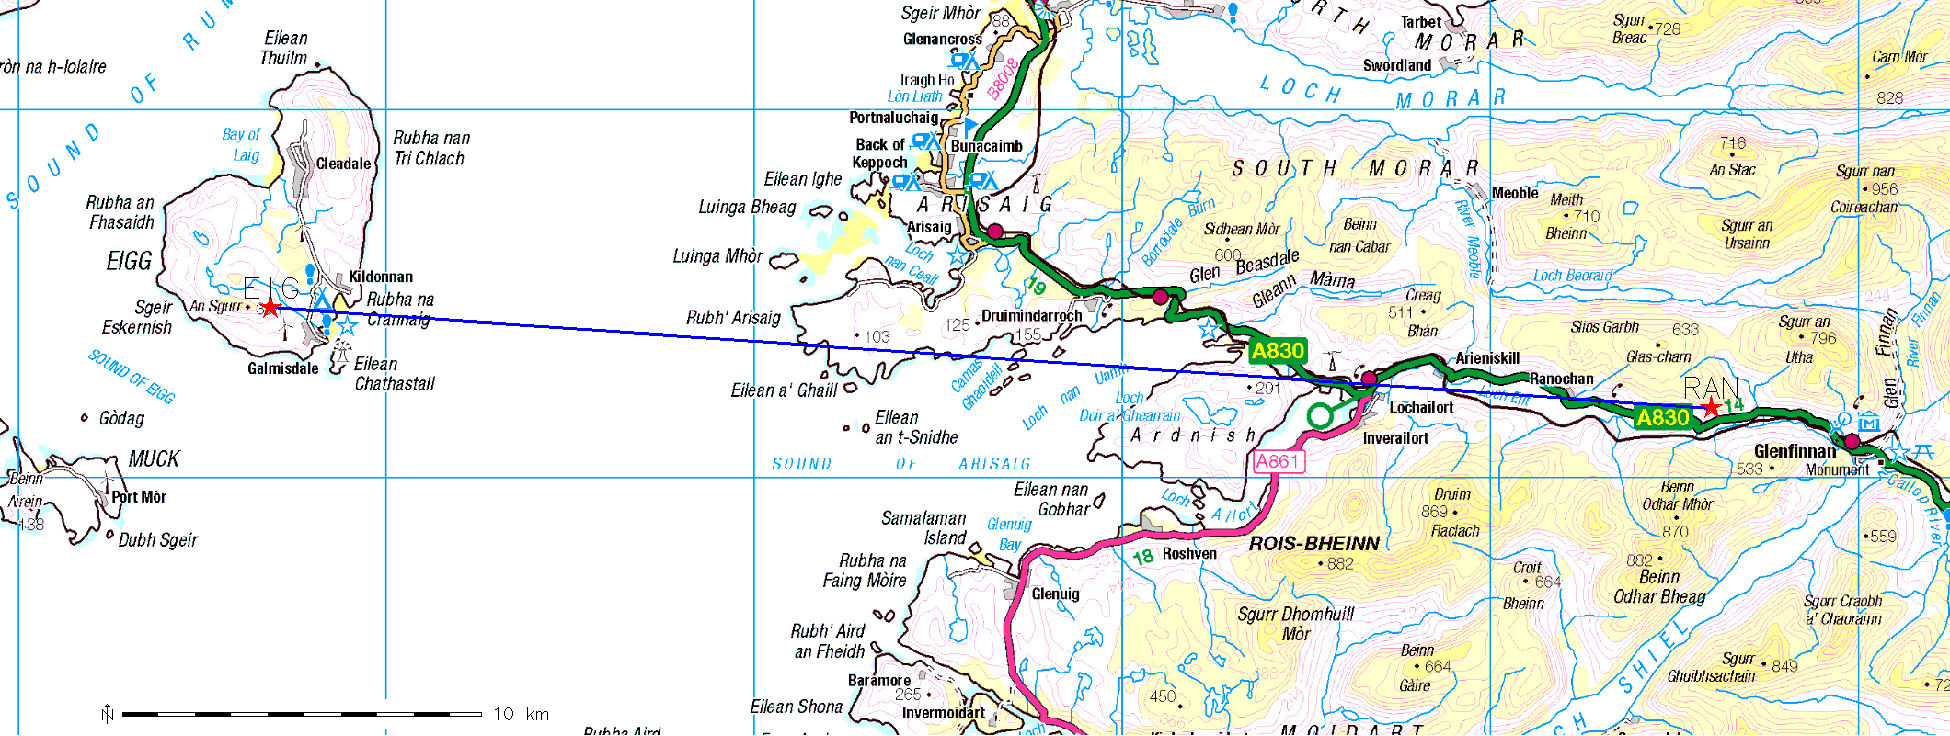
\includegraphics[width=\textwidth]{special/EIG_RAN_map.png}
  \end{center}
  \label{fig:eig_ran_map}
  \caption{Map of the Eigg to Ranachan path}
\end{figure}

Figure \ref{fig:eig_ran_map} gives an idea of what we're trying to
accomplish, a link between two places about 40km apart (actually it
turns out that they're almost exactly that distance). So the first
question is, all else being equal, in a vacuum in outer space, can we
use these radios to make a 40km link at 5GHz?

In outer space we have only path loss, which is given by
\begin{equation}
L_p = 20 \log \left(\frac{\lambda}{4 \pi R}\right)
\end{equation}
this can be derived, but it's a bit tricky and we won't do it
here. Just observe the general shape of it. The $2$ is because in
non-logarithmic form everything in the brackets is squared. We use the
logarithmic form because it means we can just add things up instead of
multiplying which is easier. The $10$ (from $2 \times 10 = 20$) is
because the numbers are all in decibels (dB), this is just convention,
but we need to be consistent. The $1/R$ is the inverse-$r^2$
loss from the radio waves spreading out in space, and the $\lambda$ is
because antennas get relatively more deaf as the wavelength gets
smaller. That's it apart from some constants that basically come from
the geometry involved.

We know the frequency (pick the middle of the band, for example) and
the speed of light, and we can work out that
\begin{equation}
\lambda = \frac{c}{f}
\end{equation}
or in this case
$$
\lambda = \frac{%
  300,000,000\, \mathrm{m}/\mathrm{s}%
}{%
  5,650,000,000\,\mathrm{hz}%
} = 0.053\, \mathrm{m}
$$

This is now enough to just directly work out $L_p$ with the help of a
pocket calculator,
$$
L_p = 20 \times \log \left( \frac{0.053}{4 \times \pi \times 40000} \right)
= -140\,\mathrm{dB}
$$

This loss is what we have to overcome assuming everything else is
perfect and ideal and lossless. Suppose we (illegally) run our Rocket
radios at the maximum output power ($27\,\mathrm{dBm}$) and use the
run of the mill $30\, mathrm{dBi}$ dishes on either end. Putting these
numbers into our link budget equation \ref{eq:link_budget}, we get:
$$
P_r = 27 + 30 + 30 - 140 = -53\, \mathrm{dBm}
$$

So that's pretty good, but to interpret this better we now have to
look at the datasheet for the radio. The relevant numbers are
reproduced in figure \ref{fig:rocket_txrx}.
\begin{figure}[h]
  \begin{center}
    \begin{tabular}{lrrr}
      Modulation & Line rate & TX power & RX sensitivity\\
      \hline
      MCS0 & $6.5\, \mathrm{Mbps}$ & $27\, \mathrm{dBm}$ & $-96\,\mathrm{dBm}$\\
      MCS1 & $13\, \mathrm{Mbps}$ & $27\, \mathrm{dBm}$ & $-95\,\mathrm{dBm}$\\
      MCS2 & $19.5\, \mathrm{Mbps}$ & $27\, \mathrm{dBm}$ & $-92\,\mathrm{dBm}$\\
      MCS3 & $26\, \mathrm{Mbps}$ & $27\, \mathrm{dBm}$ & $-90\,\mathrm{dBm}$\\
      MCS4 & $39\, \mathrm{Mbps}$ & $26\, \mathrm{dBm}$ & $-86\,\mathrm{dBm}$\\
      MCS5 & $52\, \mathrm{Mbps}$ & $24\, \mathrm{dBm}$ & $-83\,\mathrm{dBm}$\\
      MCS6 & $58.5\, \mathrm{Mbps}$ & $22\, \mathrm{dBm}$ & $-77\,\mathrm{dBm}$\\
      MCS7 & $65\, \mathrm{Mbps}$ & $21\, \mathrm{dBm}$ & $-74\,\mathrm{dBm}$\\
      MCS8 & $13\, \mathrm{Mbps}$ & $27\, \mathrm{dBm}$ & $-95\,\mathrm{dBm}$\\
      MCS9 & $26\, \mathrm{Mbps}$ & $27\, \mathrm{dBm}$ & $-93\,\mathrm{dBm}$\\
      MCS10 & $39\, \mathrm{Mbps}$ & $27\, \mathrm{dBm}$ & $-90\,\mathrm{dBm}$\\
      MCS11 & $52\, \mathrm{Mbps}$ & $27\, \mathrm{dBm}$ & $-87\,\mathrm{dBm}$\\
      MCS12 & $78\, \mathrm{Mbps}$ & $26\, \mathrm{dBm}$ & $-84\,\mathrm{dBm}$\\
      MCS13 & $104\, \mathrm{Mbps}$ & $24\, \mathrm{dBm}$ & $-79\,\mathrm{dBm}$\\
      MCS14 & $117\, \mathrm{Mbps}$ & $22\, \mathrm{dBm}$ & $-78\,\mathrm{dBm}$\\
      MCS15 & $130\, \mathrm{Mbps}$ & $21\, \mathrm{dBm}$ & $-75\,\mathrm{dBm}$\\
    \end{tabular}
  \end{center}
    \label{fig:rocket_txrx}
  \caption{Transmit power and receive sensitivity for Ubiquiti Rocket
    M5 at different modulation rates. All $\mathrm{dBm}$ values are
    $+/-\, 2\, \mathrm{dB}$}
\end{figure}

A few observations about these figures. When using these radios with
dual-polarised antennas, we will never see the MCS0-MCS7 modulation
schemes because these are for single data streams. So the only ones of
interest are MCS8-MCS15. The transmit power that the radios are
capable of is less at the higher modulations. For example if we want
full speed, we can only transmit at $21\, \mathrm{dBm}$ -- that's four
times weaker than at full power (because $10^{0.3} \approx 2$). 

Supposing that we want as fast as possible a link, we need to adjust
our calculation above setting $P_t = 21$ and so we now get
$P_r = -59\, \mathrm{dBm}$.

Also, the receive sensitivty for the slower rates is really very good,
better than $-90\, \mathrm{dBm}$. In practice we will never see links
established with signal strengths at or near that range because of
ambient noise -- which tends to be at about that level.

The meaning of the receive sensitivity is that the receiver part of
the radio needs a signal at least that strong in order to establish a
connection at a given data rate. So we have calculated that we should
see a $P_r$ of $-59\, \mathrm{dBm}$ and we only need $-75\, \mathrm{dBm}$.
That's pretty good, there's a margin of $16\, \mathrm{dB}$ and all
else being equal the link should work.

Actually $16\, \mathrm{dB}$ is fairly thin. Typically a margin of
$20-25\, \mathrm{dB}$ is used to be confident. Remember that dishes
move in the wind, alignment never stays perfect, though manufacturing
quality is generally pretty good, it isn't perfect. The response of
the antennas is not flat over their entire operating range and they
can never be absolutely perfectly matched. There are also cable and
connector losses at either end that might run to $1.5\, \mathrm{dB}$.

But then we remember. In the UK, the power limits for the upper part
of the $5\,\mathrm{GHz}$ band are $36\, \mathrm{dBm}$. That means with
a $30\, \mathrm{dBi}$ dish, we are only allowed to run the transmitter
at $6\, \mathrm{dBm}$ not $21$. That has just eaten up our entire
margin!

So, how long a link can we do \textit{legally}? We have enough
information to work this out. Assuming a $20\, \mathrm{dB}$ margin, we
know that,
$$
-75 + 20 = 6 + 30 + 30 + 20 \times
\log \left(\frac{0.053}{4 \times \pi \times R} \right)
$$
rearranging,
$$
R = \frac{%
  0.053
}{%
  4 \times \pi \times 10^{\left(-75 + 20 - 6 - 30 - 30\right)/20}%
} = 4732\, \mathrm{m}
$$
Yes, that's $4.7\, \mathrm{km}$. Using bigger $34\, \mathrm{dBi}$
dishes improves this to about $7.5\, \mathrm{km}$. With a thinner
margin and tolerating a lower data rate at MCS12, we can eak out close
to $25\, \mathrm{km}$. Any longer than that, and rules are being
broken.

